A preliminary step is to find a suitable robot platform that enables both the development and testing of indoor Aerial SLAM methods.
A straightforward choice is to use a \textit{quadrotor helcopter}, commonly designed to be unmanned aerial vehicles (UAVs).
Their small size and extremely maneuverability allows both indoor and outdoor flight.
Furthermore, quadrotors don't require mechanical linkages to vary the rotor blade pitch angle, which simplifies the design.

Nowadays, small quadrotors with on-board stabilization can be bought off-the-shelf.
These quadrotors make it possible to shift the research from basic control of the platform towards intelligent applications.
The platform selected is the Parrot AR.Drone\footnote{\url{http://ardrone.parrot.com}} quadrotor helicopter.
The main advantages of this quadrotor are the robustness and affordable pricetag.
The AR.Drone is equipped with a front-camera and a down-looking camera that provide live video streaming.
Furthermore, the AR.Drone is equipped with an ultrasound sensor and an inertial unit that measures pitch, roll, yaw and accelerations along all axes.
The vehicle is controlled by sending commands over a Wi-Fi connection.

In this chapter, the AR.Drone is evaluated as a robotic platform.
The flight control of a quadrotor is described and the AR.Drone's hardware is listed.
The intelligence onboard of the vehicle is described.
Moreover, the open Application Programming Interface (API) is examined.



% Quadrotor flight control
\section{Quadrotor flight control}
% http://www.stanford.edu/~haomiao/papers/ICRA09AeroEffects.pdf
% http://www2.engr.arizona.edu/~sprinkjm/research/c2wt/uploads/Main/QuadrotorDynamicsGNC.pdf
The mechanical structure of a quadrotor consists of four rotors attached to a body frame (see Figure \ref{fig:QuadRotorBody}).
Each pair of opposite rotors (pair ${1, 3}$ and pair ${2, 4}$) is turning the same direction.
One pair is turning clockwise and the other counter-clockwise.
Each rotor produces both a thrust $T$ and torque $\tau$ about its center of rotation, as well as a drag force $D_b$ opposite to the vehicle's direction of flight.
Thrust $T$ is a force that is generated by expelling or accelerating mass in one direction.
The accelerated mass will cause a force of equal magnitude but opposite direction on that system.
Torque $\tau$ is the tendency of a force to rotate an object about an axis.
Drag $D_b$ is the force that opposes the motion of an aircraft through the air.
This force depend on velocity of the vehicle and deaccelerates the vehicle if insufficient thrust is generated.
Together the motors should generate sufficient vertical thrust to stay airborne, which is indicated by the gravity force $mg$ in the direction $e_D$.

% TODO: diagram of roll, pitch, yaw

\begin{figure}[htb]
\centering
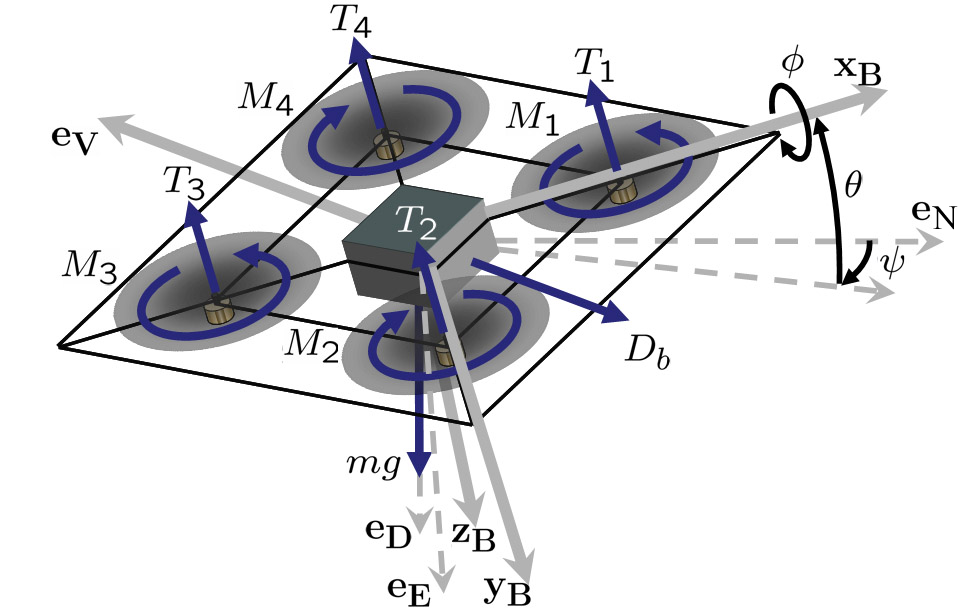
\includegraphics[width=7cm]{images/QuadRotorBody.png}
\caption{Free body diagram of a quadrotor helicopter 
%(Courtesy Hoffman \textit{et al.}
\cite{Hoffmann2007}. Note that a right-handed orthogonal coordinate system is used with the $z$-axis pointing down. Each of the 4 motors has a thrust $T_i$ and momentum $M_i$. Together the motors should generate sufficient vertical thrust to stay airborne, which is indicated by the gravity force $mg$ in the direction $e_D$. Differential thrust between the motors can provide roll $\phi$ and pitch $\theta$ torques, which lead to an angle of attack $\alpha$. This can result in fast movements of the helicopter (e.g. in the horizontal plane) in the direction $e_V$ which a resulting drag force $D_b$. }
\label{fig:QuadRotorBody}
\end{figure}

For movements, the quadrotor relies solely on differential torque and thrust.
If all rotors are spinning at the same angular velocity, the differential torque is zero, resulting in no angular acceleration about the yaw axis.
Varying the angular velocity of each rotor pair yields angular acceleration about the yaw axis.
If the total thrust is kept constant, the vertical velocity remains unchanged.
A vertical movement is achieved by increasing or decreasing the thrust from each motor by the same amount, so that total thrust changes but differential torque on the body remains zero. 
A horizontal movement is achieved by maintaining a non-zero pitch $\theta$ or roll angle $\phi$.
Angular accelerations about the pitch and roll axes can be caused separately.
Each pair of blades rotating in the same direction controls one axis, either roll or pitch.
Increasing thrust for one rotor while decreasing thrust for the other will maintain the torque balance needed for yaw stability and induce a differentie torque about the roll or pitch axes. 

\begin{comment}
\begin{figure}[htb]
\centering
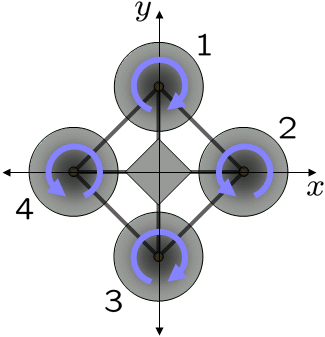
\includegraphics[width=7cm]{images/Quadrotor_yaw_torque.png}
\caption{Schematic of reaction torques on each motor of a quadrotor helicopter. Rotors 1 and 3 spin in one direction, while rotors 2 and 4 spin in the opposite direction, yielding opposing torques for control.}
\label{fig:QuadRotorRotors}
\end{figure}
\end{comment}

% Hardware
\section{Hardware}
The AR.Drone is remote-controlled consumer quadrotor helicoptor developed by Parrot SA\footnote{\url{www.parrot.com}}.
The body is made of carbon fiber tube structure and high resistance 
%PA66
plastic.
A protection hull is made of Polypropylene Foaming Material.
This hull provides protection during indoor flights.
The propellors are powered by four brushless motors (35,000 rpm, power: 15W).
Energy is provided by a Lithium polymer battery with a capacity of 1000 mAh, which allows a flight time of approximately 10 minutes.

The AR.Drone carries an internal computer with an 468MHz ARM9-processor and 128MB of RAM, running a custom Linux operating system.
An integrated 802.11g wireless card provides network connectivity with an external device that controls the vehicle.
No remote-control is provided. Instead, a regular wifi-enabled device can be used to control the AR.Drone.
It was initially designed for the Apple platforms (e.g., iPhone, iPod and iPad) and became available on other platforms in the last few months.
It is also possible to control the AR.Drone from a Linux or Windows PC with the software designed for application developers.



% Sensors
\subsection{Sensors}
The AR.Drone has different types of sensors.
These sensors are used for automatic stabilization.
In addition, a front camera is present to provide the user visual feedback from the vehicle.


\subsubsection{Inertial measurement unit}
The AR.Drone features an 6 degrees of freedom (DOF) inertial measurement unit.
It provides the software with pitch, roll and yaw measurements.
These measurements are used for automatic pitch, roll and yaw stabilization and assisted tilting control.
The measurement unit is a \textit{micro electro-mechanical system} (MEMS) and contains
a 3 axis accelerometer, a 2 axis gyrometer and a 1 axis yaw precision gyrometer.

The \textbf{accelerometer} is a BMA150\footnote{\url{http://www.bosch-sensortec.com/content/language1/downloads/BMA150_DataSheet_Rev.1.5_30May2008.pdf}} made by Bosch Sensortec.
%It provides three sensitivity ranges (i.e., maximum g-force it can report): $\pm 2g / \pm 4g / \pm 8g$.
An accelerometer outputs g-forces (acceleration relative to free-fall) as a quantity of acceleration.
It is based on the phenomenon that the (observed) weight of a mass changes during acceleration.
Typical MEMS accelerometer is composed of movable \textit{proof mass} with plates that is attached through a mechanical suspension system to a reference frame.
Movable plates and fixed outer plates represent capacitors. The deflection of proof mass is measured using the capacitance difference.
The accelerometer has three perpendicular axes. Each axis can only measure acceleration in the direction of the axis.
%The tiny micro-structures can only measure force in a single direction, or axis of acceleration.
%This means with a single axis measured, you can only know the force in either the X, Y, or Z directions.
An accelerometer at rest relative to the Earth's surface will indicate approximately 1 g upwards, because any point on the Earth's surface is accelerating upwards relative to the local inertial frame.
To obtain the acceleration due to motion with respect to the Earth, this gravity offset must be subtracted and corrections for effects caused by the Earth's rotation relative to the inertial frame.
Since the accelerometer can measure gravity, it can be used as a tilt sensor.

The AR.Drone has a 2 axis \textbf{gyrometer} and a 1 axis yaw precision gyrometer.
The gyrometer measures angular velocity in degrees per second, based on the principles of angular momentum.
In order to estimate the absolute angle $\theta$, the angular velocity signal $\Omega$ needs to be integrated with respect to time.
A major problem with this method is that bias errors in the angular velocity signal will cause the integrated angle value to drift over time, since all gyroscopes have at least a small amount of bias error in their angular rate signal.

Regular gyroscopes use a spinning wheel.
However, a small device like the AR.Drone cant afford to have a spinning wheel.
Instead, a tiny MEMS gyroscope is used. 
%In a MEMS gyroscope, two proof masses vibrate in plane at certain frequency.
It comprises of a plate, called the \textit{proof mass}, that vibrates (oscillates).
%when a drive signal is applied to set of drive capacitor plates.
When the vehicle rotates, the proof mass gets displaced in the X, Y, and Z directions by Coriolis forces.
A processor senses the proof mass’ displacement through capacitor plates located underneath the proof mass, as well as finger capacitors at the edges of the package.
The AR.Drone uses a IDG-500 Dual-Axis\footnote{\url{http://www.sparkfun.com/datasheets/Components/SMD/Datasheet_IDG500.pdf}} gyroscope for the X and Y axis of the drone.
The IDG-500 gyro has two separate outputs per axis for higher speed motions (range: $500^{\circ}/s$, sensitivity: $2.0mV/^{\circ}/s$) and lower-speed precise movements (range: $110^{\circ}/s$, sensitivity: $9.1mV/^{\circ}/s$).
The yaw orientation is measured using a high precision gyrometer: Epson Toyocom XV-3500CB\footnote{\url{http://www.eea.epson.com/portal/pls/portal/docs/1/424992.PDF}}.
%This sensor has a range of $100^{\circ}/s$
%Vibrating structure gyroscopes are simpler and cheaper than conventional rotating gyroscopes of similar accuracy
%The output is a rate of rotation about the X and Y axis.


\subsubsection{Ultrasound altimeter}
An ultrasound sensor provides altitude measures for automatic altitude stabilization and assisted vertical speed control.
The ultrasound sensor is attached on the bottom of the AR.Drone and points downwards in order to measure the distance to the floor.
A packet of ultrasonic soundwaves is transmitted towards the floor, which reflects the sound back to the sensor.
The system then measures the time $t$ for the echo to return to the sensor and computes the distance $d$ to the target using the speed of sound, using:
\begin{equation}
d = \frac{c \times t}{2}
\end{equation}
where $c \approx 343\small{m/s}$ is the speed of sound in air.

Altrasound range measurements suffer from some fundamental drawbacks which limit the usefulness.
These drawbacks are inherent to the principle of an ultrasonic sensor and their commonly used wavelengths.
\cite{borenstein1988obstacle} Describes some of these drawbacks in the context of obstacle avoidance.
A limitation is the small range in which the sensor is able to operate.
The ultrasound sensor in the AR.Drone has a effective range of approximately $20\small{cm}$ to $6\small{m}$.
%The minimum range is approximately $20\small{cm}$, meaning that the AR.Drone is \textit{unable to determine its altitude} when flying close to the floor.
Another limitation is that the ultrasound sensor is unable to obtain precise directional information about objects.
Sound progragates in a cone-like manner, where opening angles are commonly between 20 to 40 degrees.
Due to this property, the sensor acquires entire regions of constant depth instead of discrete depth points.
So, the ultrasound sensor can only tell there is an object at the measured distance somewhere within the measured cone.

Another limitation is the influence of the surface's orientation on the sensor's performance.
When the ultrasoundwave is emitted toward a parallel surface of an obstacle, most of the sound energy is reflected perpendicular to the surface and will be detected by the sensor.
However, if the surface of the obstacle is tilted relative to the sensor, then only an undetectably small amount of energy will be reflected toward the sensor.
Also, the acoustic properties of the material in range have direct impact on the sensor's performance (e.g., foam can acoustically absorb the soundwaves).
A final limition is the limited operating frequency.
Before a soundwave can be emitted, the previously emitted soundwave has to be detected by the sensor.
This reduces the minimal operating speed of the AR.Drone's ultrasound sensor to $300 / (2 \times 6) = 25\small{Hz}$.

\begin{center}
\line(1,0){250}
\end{center}
\color{mediumgray}
\small

The opening angle of the AR.Drone's ultrasound sensor is not documented.
A small experiment has been performed to determine the opening angle.

The AR.Drone was positioned at a fixed altitude of $79\small{cm}$ above a flat floor.
No obstacle was in range of the ultrasound sensor to make sure the measured altitude is the actual altitude of the AR.Drone.
The altitude measured by the ultrasound sensor was $75.2\small{cm}$, which equals an acceptable error of $3.8\small{cm}$.
The AR.Drone's bottom camera was used to mark a point on the floor that is exactly below the center of the AR.Drone.
This point is equal to the center of ultrasound cone.
In order to measure the opening angle, floating objects were moved from outside the cone towards the cone.
The objects require a certain distance from the floor to achieve a distance short than the shortest distance between the sonar and the floor.
The minimal altitude of an object when assuming a maximum opening angle of 40 degrees is:
\begin{equation}
a = 79\small{cm} - (cos(40\deg) \times 79\small{cm}) = 18.48\small{cm}
\end{equation}
Fluctuations in the altitude measurements indicate that the object is entering the cone.
The horizontal distance $d$ between the object and cone center (marked point) is the width of the cone and $h = 79\small{cm} - a$ is the height of the cone.
The angle $\alpha$ of the cone can be recovered with:
\begin{equation}
\alpha = tan^{-1}(d / h)
\end{equation}

The experiment was repeated 10 times with different objects.
The average opening angle is $25.03^{\circ}$ with a standard deviation of $1.45^{\circ}$.
\normalsize
\normalcolor


\begin{center}
\line(1,0){250}
\end{center}
\color{mediumgray}
\small

During flight, the AR.Drone can take a broad range of angles (the default maximum angle of attack is $12^{\circ}$).
The floor is not always perpendicular to the orientation of the ultrasound sensor, which may influence the altitude measurements.
A small experiment was performed to measure the effect of the AR.Drone's angle of attack $\alpha$ and the error $\epsilon$ of the measured altitude.

This experiment was performed above a flat floor.
The angle of attack $\alpha$ was changed slowly while keeping the AR.Drone at a fixed altitude.
A relation between the angle $\alpha$ and measured altitude was observed.
The following (first degree) polynomial fit describes the relation between the angle $\alpha$ and error $\epsilon$ of the measured altitude:
\begin{equation}
\epsilon = 0.2214 \times \alpha \hspace{0.2cm} \small{cm}
\end{equation}
\normalsize
\normalcolor



\subsubsection{Camera's}
The AR.Drone is equipped with two CMOS camera's: a front camera and a bottom camera.
Both camera's support live video streaming at 15 frames per second.

The front camera has a resolution of $640 \times 480$ pixels (VGA) and a wide $93^{\circ}$ field of view.
This front camera is used to automatically detect other drones during multiplayer games or to provide video feedback on a screen (e.g., smartphone).
The bottom camera has a resolution of $176 \times 144$ pixels (QCIF) and a $60^{\circ}$ field of view.
The video frequency of this camera is 60 frames per second to reduce motion blur and improve the applicability of intelligent algorithms.
Despite the high frequency, the frames are streamed at 15 frames per second.

\textit{front + bottom camera sample}

The bottom camera plays a central role in the AR.Drone's onboard intelligence.
It is used for horizontal / vertical stabilization (i.e., automatic hovering and trimming) and to estimated the velocity of the drone.
More details about the onboard intelligence can be found in Section \ref{sec:platform_onboard_intelligence}.



% Onboard intelligence
\section{Onboard intelligence}
\label{sec:platform_onboard_intelligence}
Usually quadrotor remote controls feature levers and trims for controlling pitch, roll, yaw and throttle.
It generally takes hours of practice to safely perform basic manoeuvres like take-off, trimming, hovering with constant altitude, and landing.
Thanks to the onboard computer and sensors, take-off, hovering, trimming and landing are now completely automatic and all manoeuvres are completely assisted.
The AR.Drone has several sources of information available about its movements and the majority of its computing power is dedicated to combine these sources into combined estimates.

\subsection{Sensor filtering and fusion}

\subsection{Wireless transmission of sensor data and video}

\subsection{Take-off and lading}

\subsection{Hovering}
	%Active deacceleration

\subsection{Trimming}

%\subsection{Active deacceleration}

%\subsection{Enemy detection}








	

% Open application programming interface
\section{Open Application Programming Interface}


%\subsection{Sensor data}